\documentclass[8pt]{beamer}
\usepackage{tikz}
\usepackage[utf8]{vietnam}
\usepackage{amsmath}
\usepackage{graphicx}
\usepackage{wrapfig}
\usepackage{hyperref}
\usetheme{Copenhagen}
\usecolortheme{beaver}
\setbeamertemplate{navigation symbols}{}
\setbeamertemplate{headline}{}
\title[Chương 1: Tín hiệu và hệ thống] %optional
{Chương 1: Tín hiệu và hệ thống}
\subtitle{Tín hiệu và hệ thống}
\author[Tín hiệu và hệ thống] % (optional)
{Tín Vũ}
\date[VLC 2021] % (optional)
{tinvu1309@gmail.com}
\begin{document}
\frame{\titlepage}
\begin{frame}{Mục lục}
\tableofcontents
\end{frame}
\begin{frame}{Giới thiệu playlist}
\section{Giới thiệu playlist}
	\begin{itemize}
		\item Mình là Tín Vũ, hiện tại đang là sinh viên học tại Trường Đại học Công nghệ, Đại học Quốc gia Hà Nội. Mình tạo playlist video này để hỗ trợ các bạn học môn Tín hiệu và hệ thống trong các trường đại học kĩ thuật theo hướng \alert{trực quan hóa} nhất có thể.
		\item Do đó, mục tiêu của mình khi thực hiện playlist này không chỉ giúp các bạn ôn thi được điểm cao mà còn \alert{hiểu sâu công thức để làm nền tảng cho các môn học sau}.
		\item Để đạt được hai mục tiêu trên, các bạn nên xem \textbf{toàn bộ} video của mình, còn nếu chỉ cần ôn thi cấp tốc và đạt điểm cao thì hãy \textbf{bỏ qua} các video "optional".
		\item Nội dung playlist này chủ yếu bám sát nội dung môn học Tín hiệu và hệ thống tại trường của mình; nếu các bạn học trường khác, hãy tham khảo kĩ đề cương hay đề thi của trường bạn để đối chiếu sao cho ôn tập đúng trọng tâm và hợp lý. 
		\item Môn học này bao gồm \textbf{6} chương, các chương đều liên quan rất chặt chẽ và logic với nhau nên hãy học cẩn thận ngay từ \alert{chương 0} để ôn thi cuối kì đỡ vất vả.
	\end{itemize}
\end{frame}
\begin{frame}{Tài liệu tham khảo}
\section{Tài liệu tham khảo}
\begin{itemize}
		\item Tài liệu tham khảo chính: Signals and Systems (2nd edition) Alan V. Oppenheim and Alan S. Willsky.
		\item Tài liệu tham khảo phụ: Bài tập của mình học khóa trước, đề thi các năm cũ,...
		\item Tài liệu tham khảo phụ: Nếu bạn là sinh viên trường mình và muốn học "tủ" nhiều bài thì nên đọc Signals and Systems (2nd edition) Simon Haykin vì các thầy cô chủ yếu dạy và ra đề trong cuốn này, thế nhưng mình đánh giá cuốn này không đầy đủ và chi tiết như sách của Alan V. Oppenheim. 
	\end{itemize}
\end{frame}
\begin{frame}{Tín hiệu}
	\section{Tín hiệu}
\subsection{Tín hiệu là gì ?}
\begin{itemize}
	\item Tín hiệu là gì ?
\end{itemize}
Trước khi trả lời câu hỏi trên, trước tiên chúng ta hãy thử tự tìm ví dụ của "tín hiệu" trong cuộc sống, sau đó ta mới tìm điểm chung giữa chúng và khái quát hóa lại thành một định nghĩa rõ ràng. Rất dễ để thấy được ngay các ví dụ như sau: tín hiệu đèn giao thông, tín hiệu từ các mạch điện tử, tín hiệu cơ học như sóng âm thanh từ người thương chẳng hạn,... 
\begin{figure}[h]
			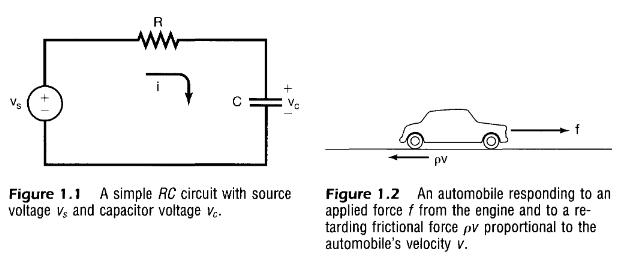
\includegraphics[width=0.6\textwidth]{signal.jpg}
			\caption{Example of signals in and out}			\label{fig:re1}
		\end{figure}
	Ta có thể thấy rằng các tín hiệu quen thuộc kể trên đều có đặc điểm chung là \textbf{đều có thể biểu diễn bằng hàm số đơn hoặc đa biến, trong đó có biến thời gian}, và \textbf{đều mang thông tin}. Trong giới hạn của môn học này, chúng ta chỉ xét đến dạng tín hiệu cơ bản nhất, được định nghĩa là \alert{một hàm số đơn biến theo biến thời gian}.
\end{frame}
\begin{frame}{Tín hiệu}
\subsubsection{Tín hiệu liên tục là gì ?}
\begin{itemize}
	\item[-] Tín hiệu liên tục là gì ?
\end{itemize}
Như đã đưa ra trong các ví dụ ở trên, chúng ta có thể thấy rằng tín hiệu liên tục xuất hiện cực kì nhiều trong thực tế, và chúng đều là hàm số theo biến \textbf{thời gian liên tục $t$}. Vậy chúng ta định nghĩa \alert{tín hiệu liên tục là tín hiệu theo hàm của biến số thời gian liên tục, tức là hàm số theo biến $t$}. 
\subsubsection{Tín hiệu rời rạc là gì ?}
\begin{itemize}
	\item[-] Tín hiệu rời rạc là gì ?
\end{itemize}
Tương tự như khái niệm của tín hiệu liên tục, chúng ta định nghĩa \alert{tín hiệu rời rạc là tín hiệu theo hàm của biến số thời gian rời rạc, tức là hàm số theo biến $n$}. Khác với tín hiệu liên tục là tín hiệu tự nhiên, tín hiệu rời rạc là tín hiệu nhân tạo được con người tạo ra thông qua quá trình \textit{lấy mẫu (sampling)} tín hiệu liên tục. 
\\ Ví dụ: khi cho máy tính phân tích một tín hiệu âm thanh liên tục, nó sẽ \textit{lấy mẫu} tín hiệu âm thanh này để "rời rạc hóa" dữ liệu rồi sau đó mới có thể sử dụng các thuật toán như \alert{Fast Fourier Transform} để xử lý. 
  \begin{figure}[h]
			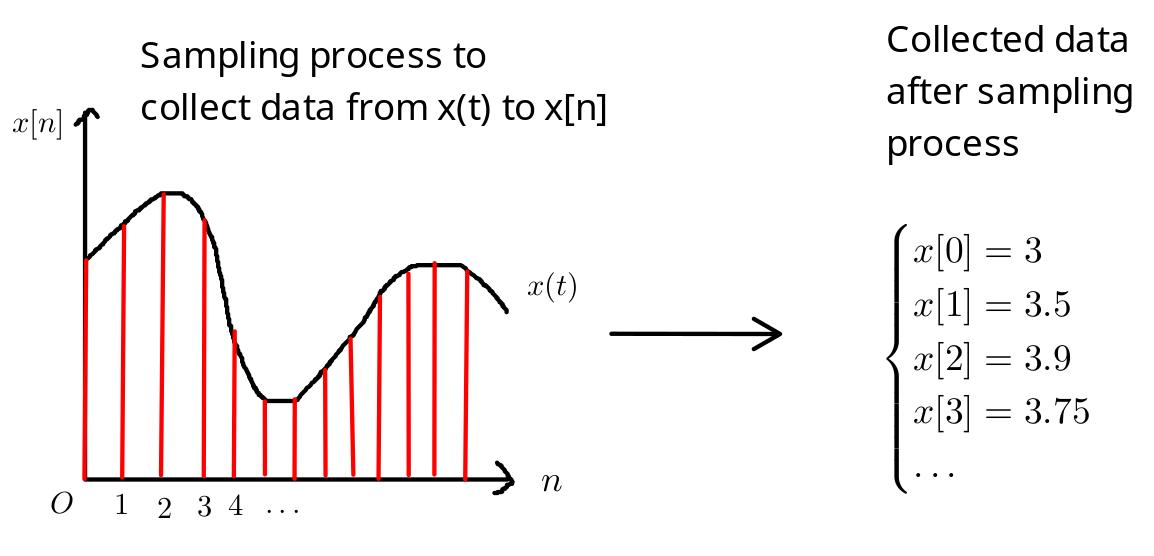
\includegraphics[width=0.6\textwidth]{sample.jpg}
			\caption{Sampling process}			\label{fig:re2}
		\end{figure}
\end{frame}
\begin{frame}{Tín hiệu}
Suy ngẫm: $n$ có thể \textbf{không} nguyên hay không ? Các hệ thống máy tính \textit{số} có nhất thiết \textbf{phải} rời rạc hóa tín hiệu trước khi xử lý chúng hay không ? Giải thích câu trả lời.
\subsection{Tín hiệu liên tục}
\subsubsection{Công suất và năng lượng}
\begin{itemize}
	\item Tín hiệu liên tục
\end{itemize}
	\begin{itemize}
		\item[-] Công suất và năng lượng
	\end{itemize}

Trước khi xây dựng công thức tính công suất và năng lượng của tín hiệu liên tục, ta tìm hiểu ví dụ đơn giản xét một mạch điện chỉ có điện trở $R$ như hình vẽ:
  \begin{figure}[h]
			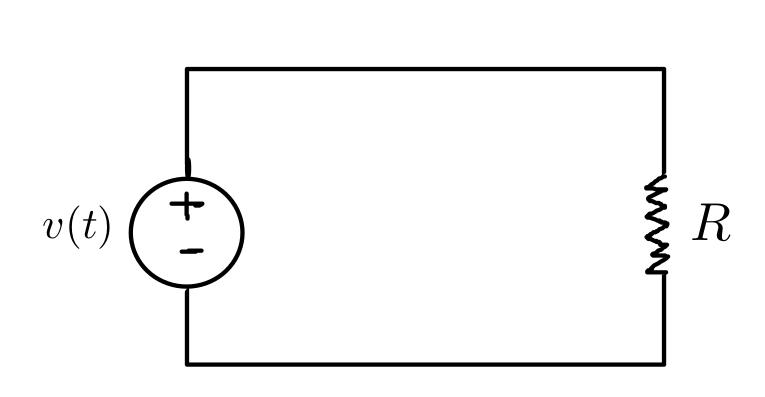
\includegraphics[width=0.6\textwidth]{r.jpg}
			\caption{Simple circuit}			\label{fig:re3}
		\end{figure}
\end{frame}
\begin{frame}{Tín hiệu}
Công suất tức thời tiêu thụ trên điện trở $R$ tại thời điểm $t$ là:
$$P_{int}=\frac{v^{2}(t)}{R}$$
Năng lượng tiêu thụ trên điện trở $R$ trong khoảng thời gian $t_{1}\to t_{2}$ là:
$$E=\int_{t_{1}}^{t_{2}}P_{int}dt=\int_{t_{1}}^{t_{2}}\frac{v^{2}(t)}{R}dt$$
Nếu tính năng lượng trên toàn miền thời gian, tức là từ $-T \to T$ với $T\to+\infty$:
$$E_{\infty}=\lim_{T\to+\infty}\int_{-T}^{T}\frac{v^{2}(t)}{R}dt=\int_{-\infty}^{+\infty}\frac{v^{2}(t)}{R}dt$$
Nếu tính công suất tiêu thụ \alert{trung bình} trên toàn miền thời gian (hay gọi tắt là công suất trong môn học này), ta xây dựng công thức từ $E_{\infty}$:
$$P_{avg}=\lim_{T\to +\infty}\frac{E_{\infty}}{T-(-T)}=\lim_{T\to+\infty}\frac{E_{\infty}}{2T}$$
Tổng quát hóa, nếu chúng ta xét năng lượng và công suất của tín hiệu $x(t)$ bất kì (cả thuần thực hoặc phức) trên toàn miền thời gian và bỏ qua hằng số, ta có công thức tính như sau:
\end{frame}
\begin{frame}{Tín hiệu}
	\begin{block}{Công thức tính năng lượng và công suất của $x(t)$ trên toàn miền thời gian}
	\begin{equation*}
		\begin{split}
			E_{\infty}&=\lim_{T\to +\infty}\int_{-T}^{T}|x(t)|^2dt=\int_{-\infty}^{+\infty}|x(t)|^2 dt \\
			P_{avg}&=\lim_{T\to +\infty}\frac{E_{\infty}}{2T} \\
		\end{split}
	\end{equation*}
	\end{block}
	Ví dụ: xác định năng lượng và công suất của hai tín hiệu sau trên toàn miền thời gian (từ giờ trở đi chúng ta quy ước chỉ gọi tắt là năng lượng và công suất) $x_{1}(t)=e^{-2t} \; (t\geq 0)$, $x_{2}(t)=\cos{(\pi t)}$:
\begin{enumerate}
	\item 
	\begin{equation*}
	\begin{split}
		E_{1}&=\int_{-\infty}^{+\infty}|x_{1}(t)|^2dt=\int_{0}^{+\infty}e^{-4t}dt=0.25 \\
		P_{1}&=\lim_{T\to +\infty}\frac{E_{1}}{2T}=0 \\
	\end{split}
\end{equation*}
\item $$x_{2}^2(t)=\cos^2{(\pi t)}=\frac{\cos(2\pi t)+1}{2}$$
\end{enumerate}
\end{frame}
\begin{frame}{Tín hiệu}
\begin{equation*}
\begin{split}
	E_{2}&=\int_{-\infty}^{+\infty}|x_{2}(t)|^2dt=\int_{-\infty}^{+\infty}\cos^2{(\pi t)}dt=+\infty \\
	P_{2}&=\lim_{T\to +\infty}\frac{E_{2}}{2T}=\frac{+\infty}{+\infty}= \; ??? \\
\end{split}
\end{equation*}
Đến đây, ta có thể thấy rõ rằng sử dụng công thức đơn thuần không tính được giá trị cụ thể của $P_{2}$. Ta thử hướng giải quyết bài toán bằng cách vẽ đồ thị trực quan từ công thức nhân đôi của hàm $\cos{}$ như sau:
\begin{figure}[h]
			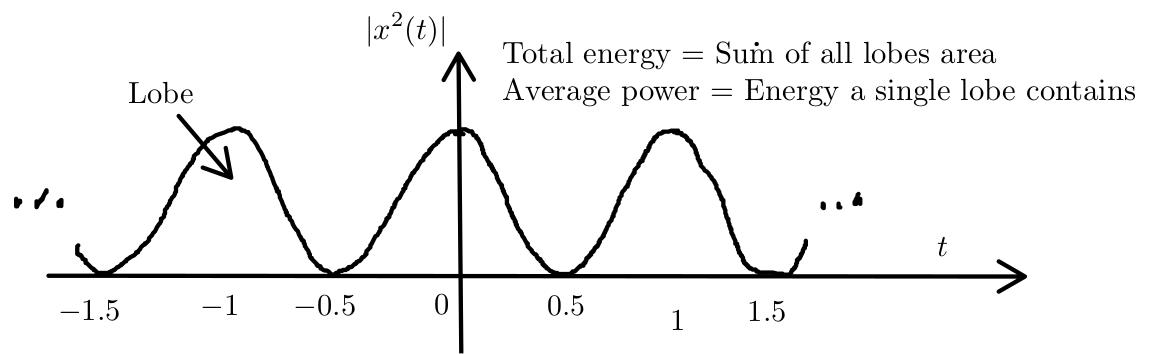
\includegraphics[width=0.8\textwidth]{lobe.jpg}
		\caption{Sketch $|x^2(t)|$ graph}			\label{fig:re4}
		\end{figure}

\end{frame}
\begin{frame}{Tín hiệu}
Để tính công suất trung bình của tín hiệu, ta chọn một "búp" $[-0.5,0.5]$ và tính năng lượng của nó:
$$P_{2}=E_{[-0.5,0.5]}=\int_{-0.5}^{0.5}\cos^2{(\pi t)}dt=0.5$$
Suy ngẫm: nếu ta lấy "búp" trên khoảng giá trị khác như $[-1.5, -0.5]$ thì giá trị $P_{2}$ có thay đổi không ? Thay vì lấy một "búp" sóng nguyên vẹn, ta sẽ lấy khoảng giá trị \textbf{vừa bằng chiều dài của một búp, tức là bằng chu kì cơ sở của tín hiệu} như $[-0.7, 0.3]$ thì $P_{2}$ thay đổi như thế nào ? Giải thích câu trả lời.
\\ Ta đưa ra $2$ khái niệm mới sau:
\begin{enumerate}
	\item Tín hiệu năng lượng là loại tín hiệu có năng lượng \alert{hữu hạn} như $x_{1}(t)$.

	\item Tín hiệu công suất là loại tín hiệu có công suất \alert{hữu hạn} như $x_{2}(t)$.
\end{enumerate}
Suy ngẫm: có tín hiệu nào đồng thời vừa là tín hiệu năng lượng, vừa là tín hiệu công suất không ? Giải thích câu trả lời.
\end{frame}
\begin{frame}{Tín hiệu}
\subsubsection{Tính tuần hoàn}
\begin{itemize}
	\item[-] Tính tuần hoàn
\end{itemize}
Một tín hiệu tuần hoàn với chu kì $T$ khi và chỉ khi:
$$x(t)=x(t+T)$$
Với $T_{0}=min(T)$ và $T_{0}$ \textbf{không âm}, ta có:
$$x(t)=x(t+T_{0})$$
Ta gọi giá trị $T_{0}$ là \alert{chu kì cơ sở của tín hiệu $x(t)$}. Một tín hiệu tuần hoàn có vô số chu kì $T$ như $\sin{(x)}\; (T=k2\pi, k \in \mathbb{Z})$, nhưng chỉ có \alert{duy nhất} một giá trị chu kì cơ sở $T_{0}$, như $\sin{(x)}$ $(T_{0}=2\pi)$. Có hai dạng tín hiệu tuần hoàn phổ biến nhất, đó là dạng \textbf{sine} và \textbf{mũ phức}.
\\ Ví dụ: xác định chu kì cơ sở của các tín hiệu sau: $x_{1}(t)=e^{j\frac{5\pi}{7}t}$, $x_{2}(t)=\cos{(3\pi t)}+\sin{(\frac{5\pi}{7}t)}$
\begin{enumerate}
	\item $$x_{1}(t)=e^{j\frac{5\pi}{7}t}=e^{j\frac{5\pi}{7}t}e^{jk2\pi}=e^{j\frac{5\pi}{7}(t+k\frac{14}{5})}\Rightarrow T_{0}=\frac{14}{5}$$
	\item $$x_{2}(t)=\cos{(3\pi t)}+\sin{\left(\frac{5\pi}{7}t\right)}$$
\end{enumerate}
\end{frame}
\begin{frame}{Tín hiệu}
Ta tìm chu kì cơ sở của từng tín hiệu thành phần cấu tạo nên $x_{2}(t)$ như sau:
\begin{equation*}
	\begin{cases}
		T_{1}=\frac{2\pi}{3\pi}=\frac{2}{3} \\
		T_{2}=\frac{2\pi}{\left(\frac{5\pi}{7}\right)}=\frac{14}{5} \\
	\end{cases}
\end{equation*}
Ta có ràng buộc tìm $m, n\in\mathbb{N}$ nhỏ nhất sao cho $mT_{1}=nT_{2}=T_{0}$, ta tìm được $m=21\; ,n=5\Rightarrow T_{0}=14$
\\Suy ngẫm: bản chất của $T_{0}$ là gì ? Tại sao ta lại có công thức ràng buộc trên ? $m, n$ có thể \textbf{không nguyên dương} được hay không và vì sao ? Giải thích câu trả lời. (Gợi ý: sử dụng đồ thị được vẽ ở slide sau gồm: $\cos{(3\pi t)}$, $\sin{\left(\frac{5\pi}{7}\right)}$, $x_{2}(t)$)
\end{frame}
\begin{frame}{Tín hiệu}

\begin{figure}[h]
			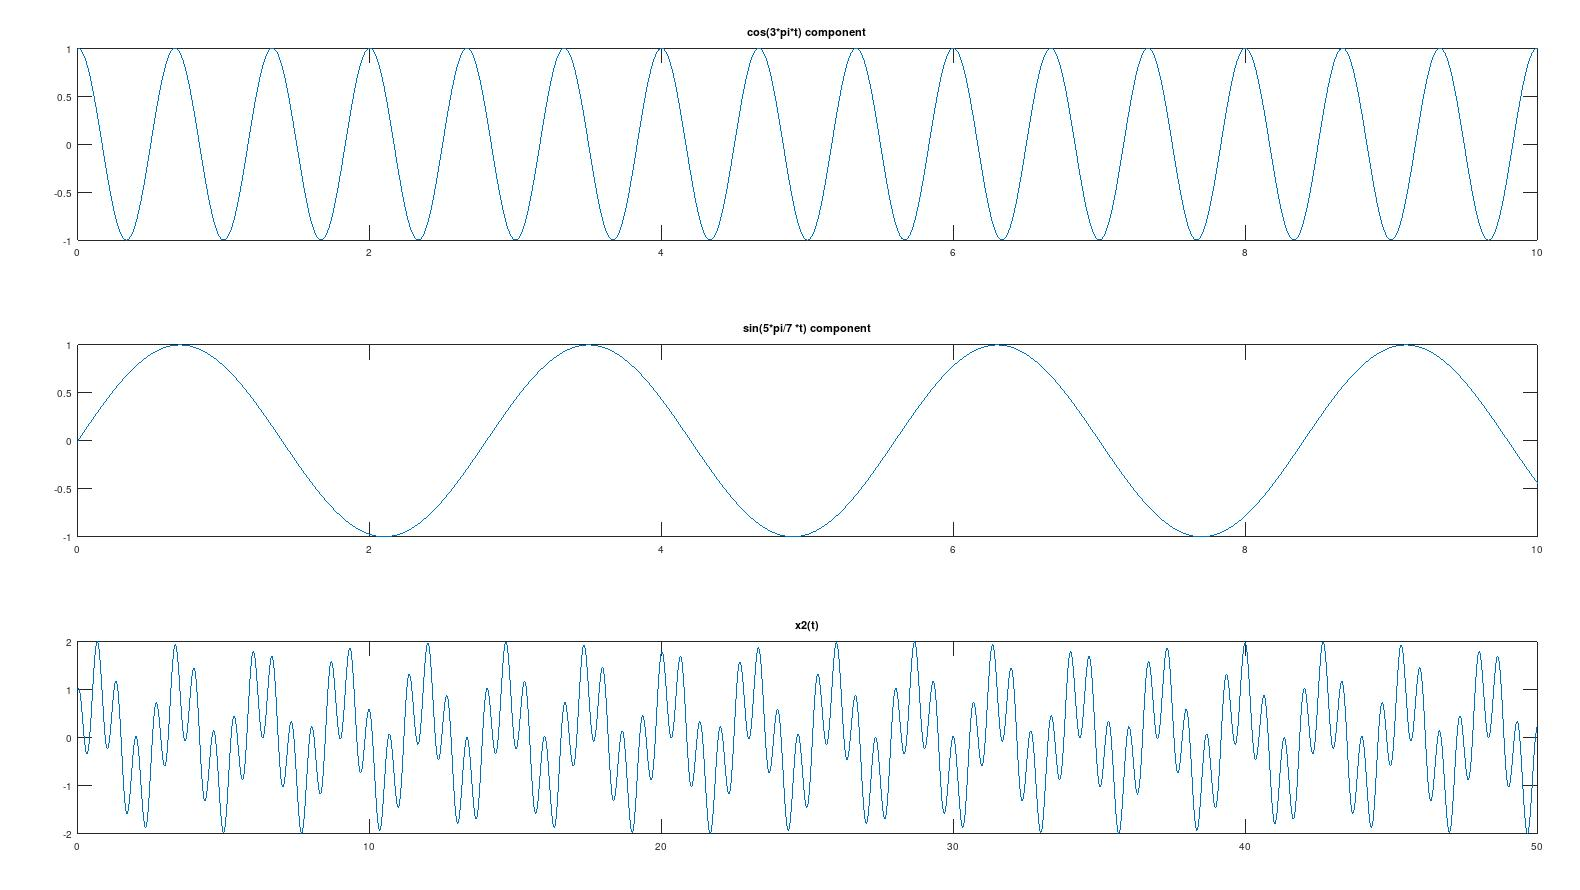
\includegraphics[width=1\textwidth]{x2t.jpg}
			\caption{Sketch $x_{2}(t)$ graph by GNU Octave}			\label{fig:re6}
		\end{figure}
	\end{frame}
\begin{frame}{Tín hiệu}
\subsubsection{Các phép toán với tín hiệu}
\begin{itemize}
	\item[-] Các phép toán với tín hiệu
\end{itemize}
Tương tự như các phép toán với hàm số, ta có bốn phép toán cơ bản với tín hiệu bao gồm \textbf{nén, giãn, lật, dịch} tín hiệu.
\begin{enumerate}
	\item Nén tín hiệu: $x(t)\to x(at) \quad (a>1)$
	\item Giãn tín hiệu:   $x(t)\to x(at) \quad (0<a<1)$
	\item Lật tín hiệu: $x(t)\to x(-t)$
	\item Dịch tín hiệu: $x(t)\to x(t-t_{0})$
\end{enumerate}
Phép biến đổi tín hiệu tổng quát (bao gồm cả $4$ phép toán) là $x(t)\to x(at+b)$.
\\ Một trong những ứng dụng cơ bản nhất của phép toán \textbf{nén} và \textbf{giãn} tín hiệu là quá trình tăng (nén) cũng như giảm (giãn) tốc độ video. Các bạn có thể thử giảm tốc độ phát video này về $x0.75$ rồi tăng lên $x2$ để khắc sâu bản chất của phép toán.  
\end{frame}
\begin{frame}{Tín hiệu}

\begin{figure}[h]
			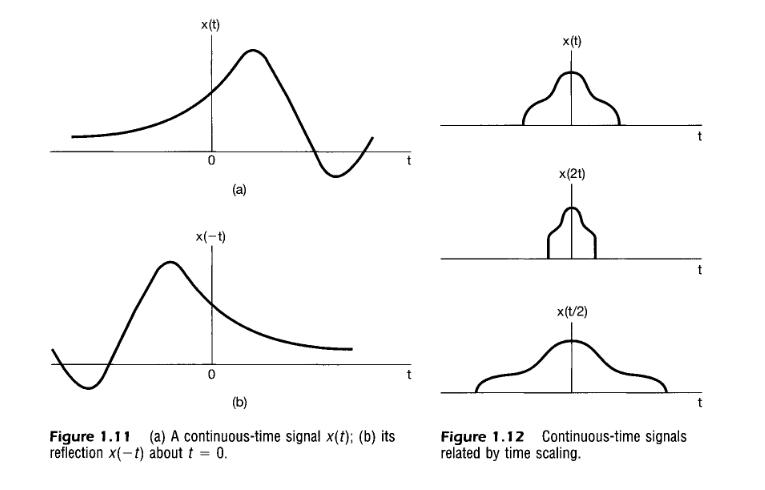
\includegraphics[width=1\textwidth]{compress.jpg}
			\caption{Example of reflection and time scaling}			\label{fig:re7}
		\end{figure}
\end{frame}
\begin{frame}{Tín hiệu}
	Ví dụ: cho tín hiệu $x(t)$ như hình vẽ, hãy vẽ lại tín hiệu $x(-t+1)$ theo quy trình sau:
	\begin{enumerate}
		\item $x(t)\to x(-t) \to x(-(t-1))$
		\item $x(t)\to x(t-1) \to x(-(t-1))$
	\end{enumerate}
\begin{figure}[h]
			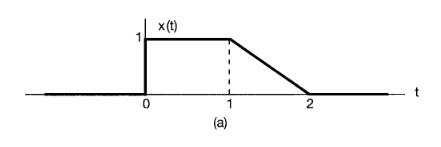
\includegraphics[width=1\textwidth]{a.jpg}
			\caption{$\text{Signal }x(t)$}			\label{fig:re8}
		\end{figure}
	\end{frame}
	\begin{frame}{Tín hiệu}
\begin{figure}[h]
			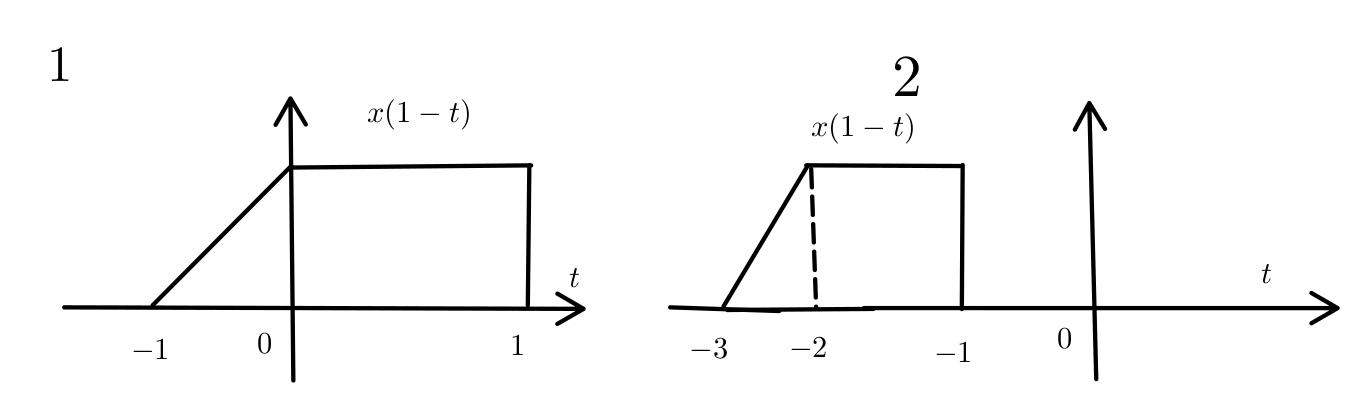
\includegraphics[width=1\textwidth]{12.jpg}
			\caption{Use process $1$ and $2$ to plot $x(1-t)$ graph}			\label{fig:re9}
		\end{figure}

	Suy ngẫm: theo bạn, tại sao $2$ quy trình trông có vẻ khá giống nhau lại cho ra kết quả khác nhau ? Điểm khác biệt mấu chốt giữa chúng là gì ? Đâu là \textbf{quy trình đúng} ? Tổng quát hóa, khi thực hiện các phép toán trên tín hiệu, chúng ta phải tiến hành theo quy trình \alert{nén/giãn rồi lật/dịch} hay \alert{lật/dịch rồi nén/giãn} ?
	\end{frame}
	\begin{frame}{Tín hiệu}
\subsubsection{Tín hiệu đơn vị}
\begin{itemize}
	\item[-] Tín hiệu đơn vị:
\end{itemize}
Cũng tương tự như khái niệm \textbf{cơ sở} của một không gian vector trong môn Đại số tuyến tính, chúng ta có thể hiểu \textbf{tín hiệu đơn vị là tín hiệu đơn giản nhất cấu tạo nên tất cả các loại tín hiệu khác}; dễ hiểu hơn nữa, chúng ta có thể hình dung tín hiệu đơn vị giống như số $0$ và số $1$ chẳng hạn, bằng các phép toán sơ cấp ta có thể vẽ được toàn bộ trục số nguyên chỉ với $2$ phần tử cơ sở. Chúng ta bắt đầu với hai tín hiệu đơn vị sau:
\begin{enumerate}
	\item Tín hiệu đơn vị nhảy bậc (unit step function)
		\begin{block}{Tín hiệu đơn vị nhảy bậc}
			\begin{equation*}
				u(t)=
			\begin{cases}
			1 \quad(t>0) \\
			0 \quad (t<0) \\
			\text{undefine} \quad (t=0)\\
		\end{cases}
	\end{equation*}
\end{block}
\item Xung Dirac đơn vị (Dirac impulse function)
	\begin{block}{Xung Dirac đơn vị}
		\begin{equation*}
			\delta(t)=
			\begin{cases}
				+\infty\quad (t=0)\\
				0 \quad \text{(otherwise)}\\
			\end{cases}
		\end{equation*}

		\end{block}
\end{enumerate}
\end{frame}
\begin{frame}{Tín hiệu}
\begin{figure}[h]
			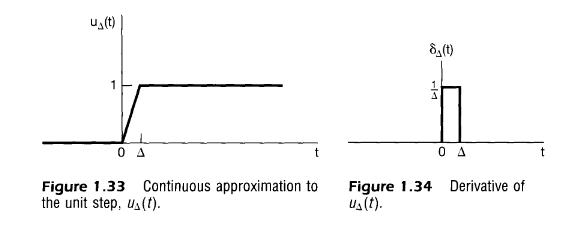
\includegraphics[width=0.7\textwidth]{unit.jpg}
			\caption{Unit step and Dirac delta function}			\label{fig:re10}
		\end{figure}


Mối liên hệ giữa $2$ tín hiệu này là:
$$\frac{du(t)}{dt}=\delta(t)\Leftrightarrow u(t)=\int_{-\infty}^{t}\delta(\tau)d\tau$$
Khi $\Delta\to 0$, quan sát hình dạng của tín hiệu $\delta(t)$, ta có thể thấy:
$$\int_{-\infty}^{+\infty}\delta(t)dt=1$$
\end{frame}
\begin{frame}{Tín hiệu}
\subsection{Tín hiệu rời rạc}
\begin{itemize}
	\item Tín hiệu rời rạc
\end{itemize}
\subsubsection{Công suất và năng lượng}
\begin{itemize}
	\item[-] Công suất và năng lượng
\end{itemize}
Cũng tương tự như tín hiệu liên tục, ta có cặp công thức sau để tính công suất và năng lượng tín hiệu rời rạc.
\begin{block}{Công thức tính năng lượng và công suất của $x[n]$ trên toàn miền thời gian}
\begin{equation*}
	\begin{split}
		E_{\infty}&=\sum_{n=-\infty}^{+\infty}|x[n]|^2 \\
		P_{avg}&=\lim_{N\to +\infty}\frac{E_{\infty}}{2N+1} \\
	\end{split}
\end{equation*}
\end{block}

Suy ngẫm: tại sao trong công thức tính công suất ta \alert{phải chia cho $2N+1$} chứ không phải $2N$ ?
\\ Ví dụ: xác định năng lượng và công suất của các tín hiệu sau trên toàn miền thời gian: $x_{1}[n]=2^{-n} \; (n\geq0)$ và $x_{2}[n]=e^{j\frac{\pi}{2}n}$.
\end{frame}
\begin{frame}{Tín hiệu}
\begin{enumerate}
	\item 
	\begin{equation*}
	\begin{split}
		E_{1}&=\sum_{n=-\infty}^{+\infty}|x_{1}[n]|^2=\sum_{n=0}^{+\infty}4^{-n}=4.333 \\
		P_{1}&=\lim_{N\to +\infty}\frac{E_{1}}{2N+1}=0\\
	\end{split}
\end{equation*}
$\Rightarrow$ Tín hiệu $x_{1}[n]$ là \alert{tín hiệu năng lượng}.
	\item 
	\begin{equation*}
	\begin{split}
		E_{2}&=\sum_{n=-\infty}^{+\infty}|x_{2}[n]|^2=\lim_{N\to +\infty}\sum_{n=-N}^{N}|x_{2}[n]|^2= \lim_{N\to +\infty}\sum_{n=-N}^{N}1=+\infty \\
		P_{2}&=\lim_{N\to+\infty}\frac{E_{2}}{2N+1}=\lim_{N\to+\infty}\frac{2N+1}{2N+1}=1 \\
	\end{split}
\end{equation*}
$\Rightarrow$ Tín hiệu $x_{2}[n]$ là \alert{tín hiệu công suất}.
\end{enumerate}
\end{frame}
\begin{frame}{Tín hiệu}
\subsubsection{Tính tuần hoàn}
\begin{itemize}
	\item[-] Tính tuần hoàn
\end{itemize}
Tương tự như tín hiệu liên tục, tín hiệu rời rạc tuần hoàn với chu kì $N$ khi và chỉ khi:
$$x[n]=x[n+N]$$
Với giá trị $N_{0}=min(N)$ và $N_{0}$ nguyên dương, ta cũng có:
$$x[n]=x[n+N_{0}]$$
Ta gọi $N_{0}$ là \alert{chu kì cơ sở của tín hiệu $x[n]$}, một tín hiệu có vô số chu kì $N$ nhưng chỉ tồn tại duy nhất một chu kì cơ sở $N_{0}$.
\\ Ví dụ: xác định chu kì cơ sở của tín hiệu $x_{1}[n]=\cos{\left(\frac{8\pi n}{31}\right)}$ và tín hiệu $x_{2}[n]=e^{j2n}$.
\begin{enumerate}
	\item
\begin{equation*}
	x_{1}[n]=\cos{\left(\frac{8\pi n}{31}\right)}=\cos{\left(\frac{8\pi n}{31}+k2\pi\right)}=\cos{\left[\frac{8\pi}{31}\left(n+\frac{31}{4}k\right)\right]}
\end{equation*}
Ta dễ thấy $N=\frac{31}{4}k$, chọn $k=4$ để thỏa mãn điều kiện $N_{0}$ nguyên dương nhỏ nhất, ta thu được $N_{0}=31$. Tương tự như tín hiệu liên tục, tín hiệu này được gọi là tín hiệu dạng \textbf{sine}.
\item 
\begin{equation*}
	x_{2}[n]=e^{j2n}=e^{j2n}e^{jk2\pi}=e^{j2\left(n+k\pi\right)}
\end{equation*}
Dễ thấy $N=k\pi$, nhưng lúc này ta \textbf{không} thể chọn được giá trị $k$ nào để $N_{0}$ nguyên dương nữa ! Vậy tín hiệu dạng \textbf{mũ phức} này không tuần hoàn.
\end{enumerate}
\end{frame}
\begin{frame}{Tín hiệu}
Suy ngẫm: có phải tất cả các tín hiệu dạng sine và mũ phức của tín hiệu rời rạc đều tuần hoàn không ? Điểm khác biệt mấu chốt với tín hiệu liên tục là gì ? Giải thích câu trả lời.
\begin{figure}[h]
			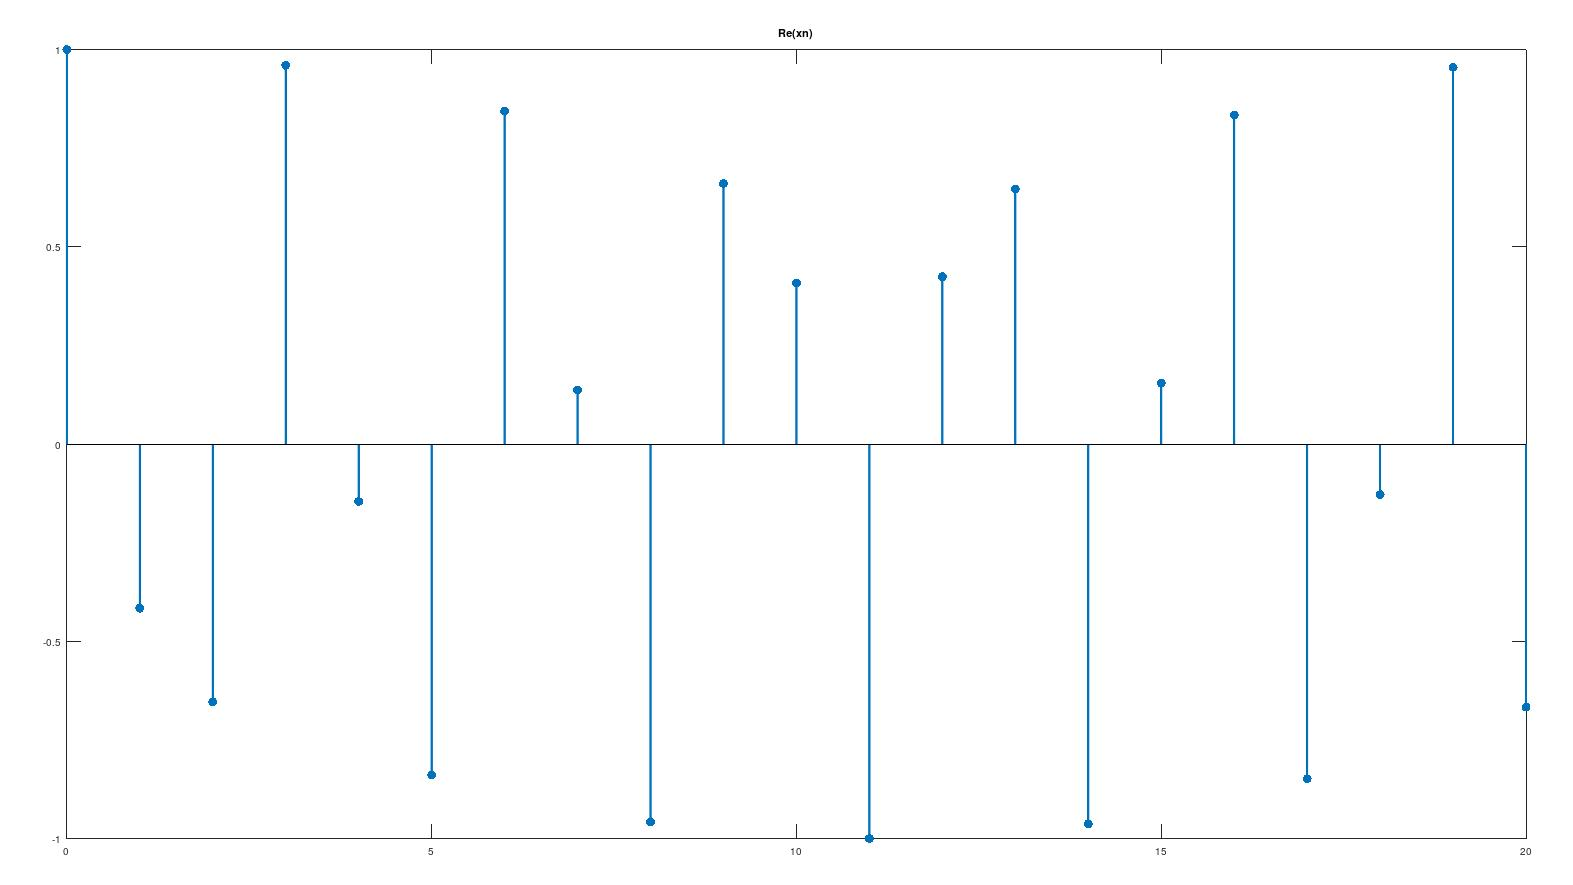
\includegraphics[width=0.9\textwidth]{re.jpg}
			\caption{Real part of $x_{2}[n]$. Do you notice it is \alert{not periodic} ?}			\label{fig:re11}
		\end{figure}
		Suy ngẫm: quan sát hình vẽ trên tại các điểm $n=3,n=4 \; (\approx \pi)$ và thử "giả vờ" tín hiệu trên tuần hoàn với chu kì cơ sở $N_{0}=3$. Nhận xét câu trả lời của bạn.
\end{frame}
\begin{frame}{Tín hiệu}
\subsubsection{Các phép toán với tín hiệu}
\begin{itemize}
\item[-] Các phép toán với tín hiệu
\end{itemize}
Tương tự với tín hiệu liên tục, tín hiệu rời rạc cũng có $4$ phép toán cơ bản gồm:
\begin{enumerate}
	\item Nén tín hiệu: $x[n]\to x[an]\quad (a>1)$
	\item Giãn tín hiệu: $x[n]\to x[an]\quad (0<a<1)$
	\item Lật tín hiệu: $x[n]\to x[-n]$
	\item Dịch tín hiệu: $x[n]\to x[n-n_{0}]$
\end{enumerate}
Phép biến đổi tín hiệu tổng quát (bao gồm cả $4$ phép toán) là $x[n]\to x[an+b]$.
\\ \textbf{Lưu ý: đối với phép nén/giãn tín hiệu rời rạc, ta luôn phải đảm bảo điều kiện $n\in \mathbb{Z}$}

\begin{figure}[h]
			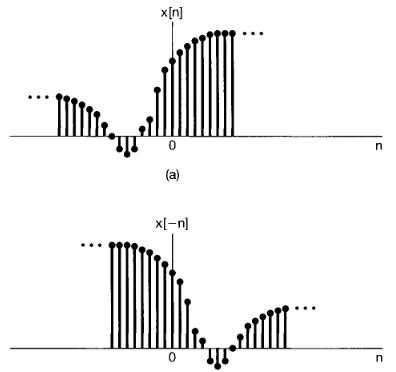
\includegraphics[width=0.4\textwidth]{reflect.jpg}
			\caption{$x[n]$ and its reflected version}	\label{fig:re12}
		\end{figure}
\end{frame}
\begin{frame}{Tín hiệu}
\subsubsection{Tín hiệu đơn vị}
\begin{itemize}
	\item[-] Tín hiệu đơn vị
\end{itemize}
Tương tự như tín hiệu liên tục, ta cũng bắt đầu với hai tín hiệu đơn vị như sau:
\begin{enumerate}
	\item Tín hiệu đơn vị nhảy bậc (unit step \textit{sequence} function)
\begin{block}{Tín hiệu đơn vị nhảy bậc}
\begin{equation*}
u[n]=
\begin{cases}
1 \quad(n\geq0)\\
0 \quad(n<0) \\
\end{cases}
\end{equation*}
\end{block}
	\item Xung Kronecker đơn vị (Kronecker impulse function)
		\begin{block}{Xung Kronecker đơn vị}
\begin{equation*}
\delta[n]=
\begin{cases}
1 \quad(n=0)\\
0 \quad(\text{otherwise)}\\
\end{cases}
\end{equation*}
\end{block}
\end{enumerate}
\end{frame}
\begin{frame}{Tín hiệu}
\begin{figure}[h]
			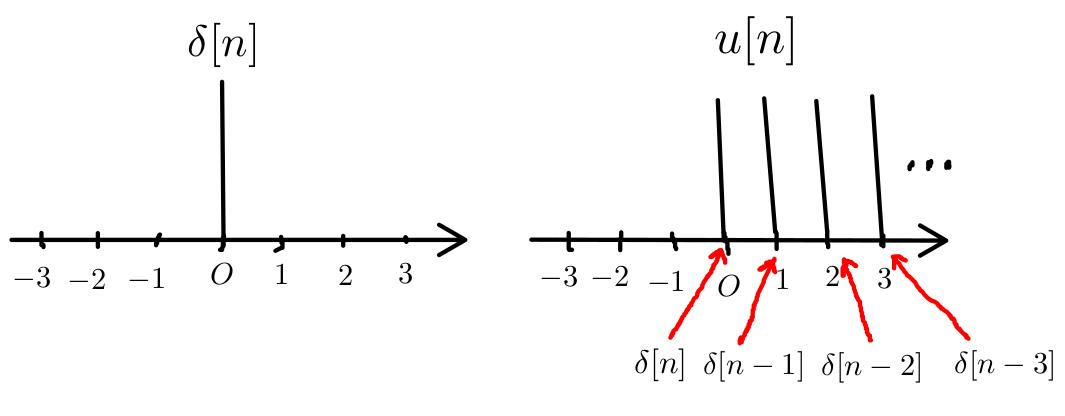
\includegraphics[width=0.9\textwidth]{kronecker.jpg}
			\caption{$\delta[n]$ and $u[n]$}	\label{fig:re14}
		\end{figure}

Từ hình vẽ trên, ta có thể dễ dàng nhìn ra được mối quan hệ của tín hiệu $\delta[n]$ và $u[n]$ là:
\begin{equation*}
\begin{split}
	u[n]&=\sum_{k=0}^{+\infty}\delta[n-k]\\
	\delta[n]&=u[n]-u[n-1]\\
\end{split}
\end{equation*}
\end{frame}
\begin{frame}{Hệ thống}
\section{Hệ thống}
\subsection{Hệ thống là gì ?}
\begin{itemize}
	\item Hệ thống là gì ?
\end{itemize}
 Trước khi trả lời câu hỏi trên, chúng ta cũng hãy bắt đầu tự thử tìm ví dụ của "hệ thống" trong cuộc sống, từ đó ta mới tìm điểm chung giữa chúng và khái quát hóa lại thành một định nghĩa rõ ràng. Như đã thảo luận ở \alert{Chương 0}, ta có thể lấy một vài ví dụ rất tiêu biểu như sau: hệ thống lọc nhiễu tín hiệu âm thanh, nhận đầu vào là \textbf{âm thanh nhiễu} và trả về đầu ra là \textbf{âm thanh "sạch"}; hệ thống khuếch đại trong các mạch điện tử chẳng hạn, nhận đầu vào là \textbf{tín hiệu có công suất thấp} và trả về đầu ra là \textbf{tín hiệu đã được khuếch đại có công suất cao},...
\\ Ta có thể nhận thấy rằng các hệ thống trên đều có đặc điểm chung là \textbf{đều nhận tín hiệu đầu vào và trả về tín hiệu đầu ra}. Trong giới hạn môn học này, chúng ta chỉ xét đến \textbf{các hệ thống vật lý} được định nghĩa là \alert{tiến trình biến đổi tín hiệu đầu vào thành tín hiệu đầu ra tương ứng}.
\\Tương tự như tín hiệu, ta cũng định nghĩa khái niệm \alert{hệ thống liên tục} và \alert{hệ thống rời rạc} như hình vẽ sau:
\begin{figure}[h]
			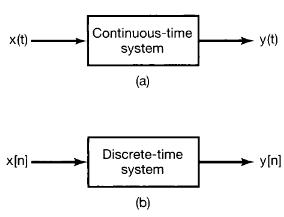
\includegraphics[width=0.4\textwidth]{system.jpg}
			\caption{$\delta[n]$ and $u[n]$}	\label{fig:re15}
		\end{figure}

\end{frame}
\begin{frame}{Hệ thống}
\subsection{Tính chất của hệ thống}
\begin{itemize}
	\item Tính chất của hệ thống
\end{itemize}
Từ slide này trở đi, chúng ta sẽ xem xét các hệ thống \textbf{liên tục} và \textbf{rời rạc} song song với nhau chứ không tách rời hai loại hệ thống như phần \alert{Tín hiệu} do các tính chất của chúng tương đối giống nhau.
\subsubsection{Tính không nhớ}
\begin{itemize}
	\item[-] Tính không nhớ
\end{itemize}
Một hệ thống được gọi là \textbf{hệ thống không nhớ} khi đầu ra của hệ thống tại thời điểm $t_{0}$ bất kì hoàn toàn chỉ phụ thuộc đầu vào của hệ thống tại thời điểm đó. Hoàn toàn tương tự với thời điểm $n_{0}$.\\ Ví dụ: hệ thống liên tục của một mạch điện tử chỉ có nguồn và điện trở $R$ với đầu vào là $x(t)$ và đầu ra $y(t)=Rx(t)$ là một hệ thống \textbf{không nhớ}; hệ thống rời rạc có quan hệ đầu ra-vào đặc trưng bởi phương trình $y[n]=x^3[n]$ cũng là một hệ thống \textbf{không nhớ}.
\\ Để chắc chắn, các bạn có thể thay thẳng giá trị $t=t_{0}$ hoặc $n=n_{0}$ bất kỳ vào phương trình đặc trưng đầu ra-vào và quan sát, nếu đầu vào chỉ xuất hiện hàm theo biến $x(t_{0})$ hoặc $x[n_{0}]$, ta có thể kết luận đây chính là hệ thống \textbf{không nhớ}.
\end{frame}
\begin{frame}{Hệ thống}
\subsubsection{Tính nhân quả}
\begin{itemize}
	\item[-] Tính nhân quả
\end{itemize}
Một hệ thống được gọi là \textbf{hệ thống nhân quả} khi đầu ra của hệ thống tại thời điểm $t_{0}$ bất kì hoàn toàn chỉ phụ thuộc đầu vào của hệ thống tại thời điểm $t_{0}$ và trước đó như $t_{0}-1$ chẳng hạn. Hay nói cách khác, \textbf{hệ thống nhân quả} là hệ thống có tín hiệu đầu ra \alert{không được phụ thuộc vào thời điểm tương lai $t_{0}$ của tín hiệu đầu vào}. Hoàn toàn tương tự với thời điểm $n_{0}$.
\\ Ví dụ: hệ thống rời rạc của bộ nhớ thiết bị điện tử là \textbf{hệ thống nhân quả}, hệ thống liên tục của mạch $RC$ với đầu vào $x(t)$ là cường độ dòng điện và đầu ra $y(t)$ là hiệu điện thế giữa hai đầu tụ $C$ có quan hệ đầu vào-ra:
$$y(t)=\frac{1}{C}\int_{-\infty}^{t}x(\tau)d\tau$$
Đây là \textbf{hệ thống liên tục nhân quả}.
Rời rạc hóa quan hệ đầu vào-ra của hệ thống này, ta cũng thu được \textbf{hệ thống rời rạc nhân quả}:
$$y[n]=\frac{1}{C}\sum_{k=-\infty}^{n}x[k]$$
Bỏ qua hằng số, ta gọi hệ thống liên tục và rời rạc thu được ở $2$ phương trình trên là \textbf{bộ tích lũy (accumulator)}.
\end{frame}
\begin{frame}{Hệ thống}
Tương tự như phương pháp xét tính không nhớ, các bạn có thể thay tùy ý giá trị $t=t_{0}$ hoặc $n=n_{0}$ vào phương trình đặc trưng đầu vào-ra và quan sát, nếu đầu vào \alert{không} xuất hiện hàm theo biến $x(t_{0}+a)$ hoặc $x[n_{0}+a]$ với $a>0$ (tức là các thời điểm tương lai tương ứng), ta có thể kết luận đây chính là hệ thống \textbf{nhân quả}.
\\ Suy ngẫm: hệ thống rời rạc sau có nhân quả hay không ? Giải thích câu trả lời.
$$y[n]=y[n+1]+x[n]$$
Gợi ý: đây là hệ thống nhân quả và là một dạng mở rộng của bộ tích lũy.
\\ Suy ngẫm: theo bạn, trong thực tế có tồn tại hệ thống không nhân quả không ? Hay hệ thống không nhân quả chỉ là một mô hình lý thuyết toán học ?
\end{frame}
\begin{frame}{Hệ thống}
\subsubsection{Tính ổn định}
\begin{itemize}
	\item[-] Tính ổn định
\end{itemize}
Một hệ thống được gọi là \textbf{hệ thống ổn định} khi ta chặn tín hiệu đầu vào bằng một hằng số $|x(t)|<B$ và ta phải chỉ ra được đầu ra cũng phải\alert{ bị chặn} bởi một hàm theo hằng số $|y(t)|<f(B)$. Hệ thống này còn được gọi là \alert{hệ thống BIBO (Bounded Input Bounded Output)}. Hoàn toàn tương tự với hệ thống rời rạc.
\\ Ví dụ: hệ thống liên tục của một mạch điện tử chỉ có nguồn và điện trở $R$ với đầu vào $x(t)$ và đầu ra $y(t)=Rx(t)$ là hệ thống \textbf{ổn định}, hệ thống rời rạc của bộ tích lũy cũng chính là hệ thống \textbf{ổn định}.
\\ Phương pháp để xét tính ổn định của hệ thống liên tục như định nghĩa gồm hai bước: đầu tiên, các bạn xét một hằng số $B$ tùy ý và tạo ràng buộc với tín hiệu đầu vào sao cho $|x(t)|<B$, sau đó tìm ràng buộc với tín hiệu ra sao cho $|y(t)|<f(B)$. Hoàn toàn tương tự với hệ thống rời rạc.
\\ Suy ngẫm: hệ thống nào sau đây ổn định và vì sao (bạn sẽ gặp lại hệ thống $1$ trong môn Điện tử tương tự và hệ thống $2$ trong môn Xử lý tín hiệu số) ?
\begin{enumerate}
	\item $$y(t)=\ln{(x(t))}$$
	\item $$y[n]=\frac{\sin{(\pi x[n])}}{\pi x[n]}$$
\end{enumerate}
\end{frame}
\begin{frame}{Hệ thống}
\begin{figure}[h]
			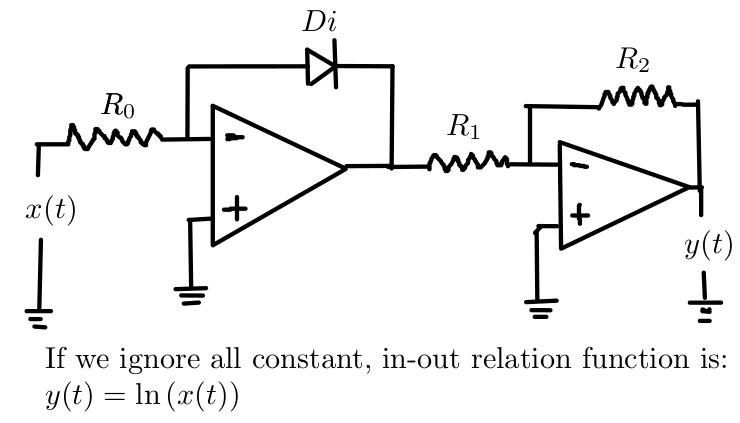
\includegraphics[width=0.5\textwidth]{loga.jpg}
			\caption{Natural logarithm circuit using Op-Amp}	\label{fig:re16}
		\end{figure}

\begin{figure}[h]
			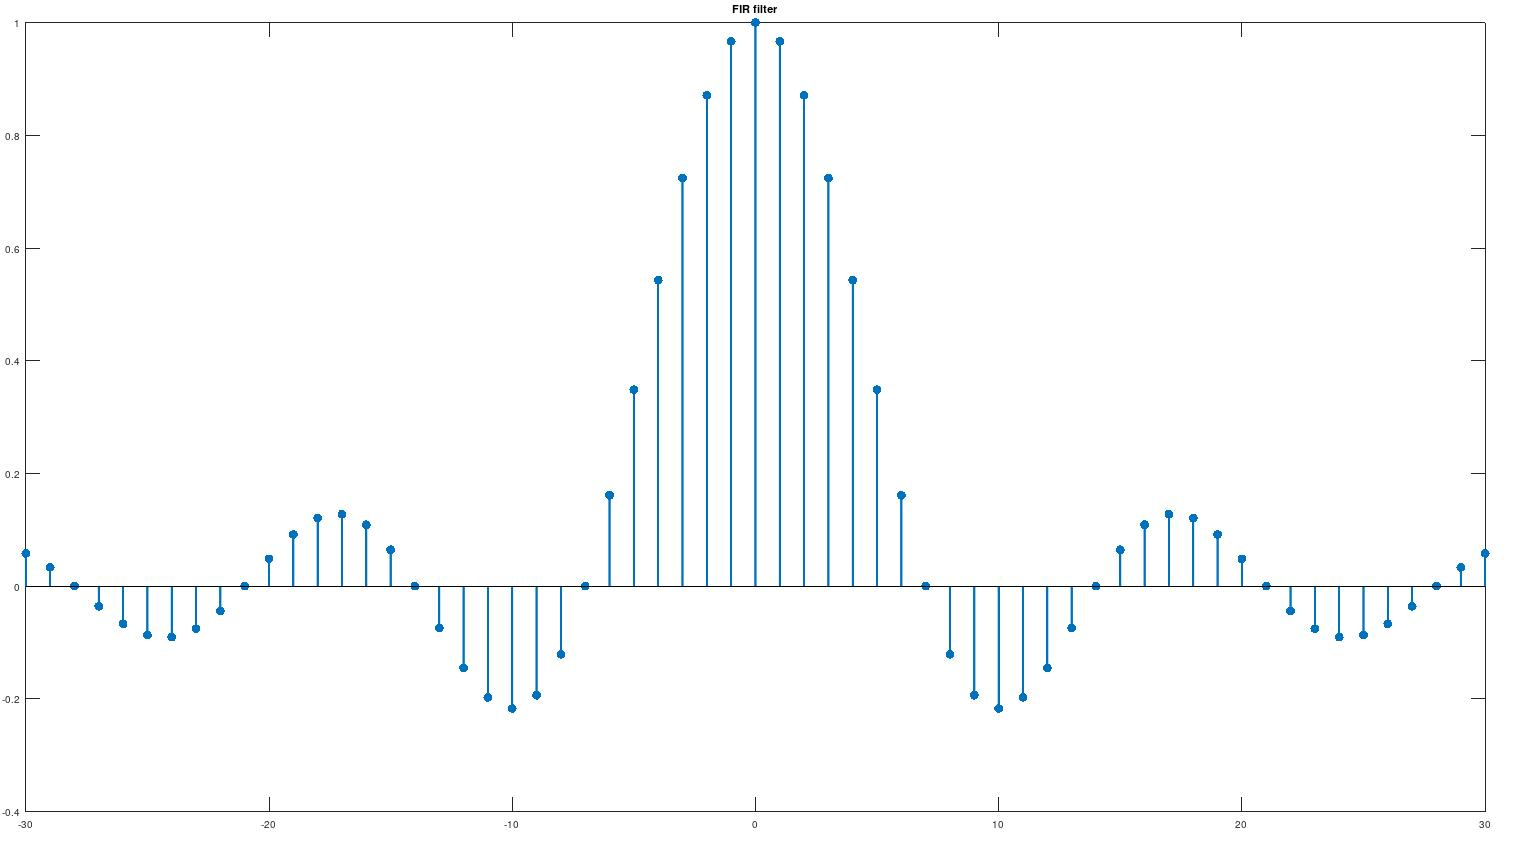
\includegraphics[width=0.5\textwidth]{fir.jpg}
			\caption{Example of FIR filter}	\label{fig:re17}
		\end{figure}
\end{frame}
\begin{frame}{Hệ thống}
\subsubsection{Tính bất biến}
\begin{itemize}
\item[-] Tính bất biến
\end{itemize}
Một hệ thống được gọi là \textbf{hệ thống bất biến} khi các đặc điểm (characteristics) và hành vi (behavior) của nó luôn \alert{cố định và không đổi theo thời gian}.
\\ Ví dụ: hệ thống liên tục của một mạch điện $RC$ có quan hệ vào-ra như đã trình bày trước:
\begin{equation}
y(t)=\frac{1}{C}\int_{-\infty}^{t}x(\tau)d\tau
\end{equation}
Hệ thống này là \textbf{hệ thống liên tục bất biến} do:
\begin{equation}
y(t-t_{0})=\frac{1}{C}\int_{-\infty}^{t-t_{0}}x(\tau)d\tau
\end{equation}
Suy ngẫm: hãy chứng minh lại công thức $(2)$. \\
Trong điều kiện các linh kiện điện tử là lý tưởng, thời điểm hiện tại ($t$) chúng ta thực hiện thí nghiệm để tìm mối quan hệ đầu vào-ra của mạch $RC$, ta thu được phương trình $(1)$. Nếu ta thực hiện lại thí nghiệm tại một thời điểm khác ($t-t_{0}$), ta phải thu được phương trình $(2)$; và đây cũng chính là cách hiểu đơn giản của khái niệm \textbf{hệ thống bất biến}: là loại hệ thống phải đảm bảo được mối quan hệ đầu vào-ra \alert{giống nhau tại tất cả các thời điểm thực hiện thí nghiệm}. Hoàn toàn tương tự với hệ thống rời rạc.
\begin{equation*}
	\begin{split}
		x(t)&\to y(t)\; \Leftrightarrow x(t-t_{0})\to y(t-t_{0}) \\
		x[n]&\to y[n]\; \Leftrightarrow x[n-n_{0}]\to y[n-n_{0}] \\
	\end{split}
\end{equation*}
\end{frame}
\begin{frame}{Hệ thống}
	Để xét tính bất biến của hệ thống, các bạn lấy hằng số $t_{0}$ hoặc $n_{0}$ và kiểm tra xem $y(x(t-t_{0}))$ và $y(t-t_{0})$ có bằng nhau không. Tương tự với hệ thống rời rạc, nếu chúng bằng nhau thì đây là \textbf{hệ thống bất biến}.
\subsubsection{Tính tuyến tính}
\begin{itemize}
	\item [-]Tính tuyến tính
\end{itemize}
Một hệ thống được gọi là \textbf{hệ thống tuyến tính} khi nó thỏa mãn \alert{nguyên lý chồng chất} (superposition principle) như sau: với $c_{i}$ là các hằng số phức tùy ý, ta có:
\begin{equation*}
	\begin{split}
		\sum_{i=0}^{m}c_{i}x_{i}(t)&\to \sum_{i=0}^{m}c_{i}y_{i}(t)\\
		\sum_{i=0}^{m}c_{i}x_{i}[n]&\to \sum_{i=0}^{m}c_{i}y_{i}[n]\\
	\end{split}
\end{equation*}
Ví dụ: hệ thống cơ học \textbf{tuyến tính} đơn giản gồm một vật thể $P$ đồng chất với \textbf{tín hiệu vào} là các vector lực $\overrightarrow{F_{0}}\; ,\overrightarrow{F_{1}}\;,\overrightarrow{F_{2}},\dots$. \textbf{tín hiệu ra} tương ứng là tổng hợp của tất cả các lực trên tại khối tâm (center of mass) của vật: $$\overrightarrow{F}=\sum_{i=0}^{n}\overrightarrow{F_{i}}$$.
\end{frame}
\begin{frame}{Hệ thống}
	Suy ngẫm: hệ thống điện học được biểu diễn trong hình vẽ dưới đây có phải hệ thống \textbf{tuyến tính} không ? Chỉ rõ \textbf{tín hiệu vào} và \textbf{tín hiệu ra}. Theo bạn, hệ thống này còn có tính chất nào khác nữa không ? Giải thích câu trả lời.

\begin{figure}[h]
			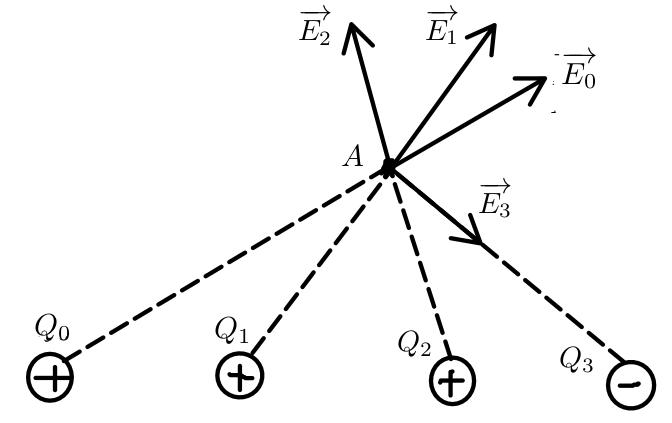
\includegraphics[width=0.5\textwidth]{e.jpg}
			\caption{Electric field}	\label{fig:re19}
		\end{figure}
Trong quá trình xét tính tuyến tính của hệ thống, để cho đơn giản, ta chỉ chọn hai hằng số phức $\alpha$ và $\beta$ chứ không nhất thiết phải chọn vô hạn số hằng số phức và chỉ ra:
\begin{equation*}
	\begin{split}
		\alpha x_{1}(t)+\beta x_{2}(t)&\to \alpha y_{1}(t)+\beta y_{2}(t) \\
		\alpha x_{1}[n]+\beta x_{2}[n]&\to \alpha y_{1}[n]+\beta y_{2}[n] \\
	\end{split}
\end{equation*}
Tất nhiên, bạn hoàn toàn có thể chọn vô hạn số hằng số phức và tiếp cận bài toán theo hướng cực kì tổng quát; như thế thì rất tuyệt vời ! Mình rất thích các lời giải tổng quát.
\end{frame}
\end{document}
